%
% Florent JACQUET - Romain THIBAUD - Antonin WALTZ
%
% Rapport de IN55 (P16)
%   Animation d'un personnage 3D avec OpenGL
%
%

\documentclass[a4paper]{report}
%packages
\usepackage[utf8]{inputenc}
\usepackage[francais]{babel}
\usepackage{graphicx}\graphicspath{{img/}}
\usepackage{float}
\usepackage[T1]{fontenc}
\usepackage{color}
\usepackage{fancyhdr}
\usepackage{listings}
\usepackage[colorlinks=true,allcolors=black]{hyperref}
\usepackage[font=small,labelfont=bf,margin=\parindent,tableposition=top]{caption}
\setcounter{tocdepth}{2}

\begin{document}
\begin{titlepage}
    
\includegraphics[width=0.4\textwidth]{logo_utbm.png}
    \begin{center}
        \textsc{\LARGE Université de Technologie de Belfort Montbéliard}\\[1cm]
        \textsc{\Large IN55}\\
        \rule{\linewidth}{0.5mm}
        { \huge \bfseries Animation d'un personnage 3D avec OpenGL\\[0.4cm] }
        \rule{\linewidth}{0.5mm}
        \vskip1cm
        % Author and supervisor
        Florent \textsc{Jacquet}\\
	Romain \textsc{Thibaud}\\
        Antonin \textsc{Waltz}\\
        Superviseur: Fabrice \textsc{Lauri}\\
        \vskip1cm
        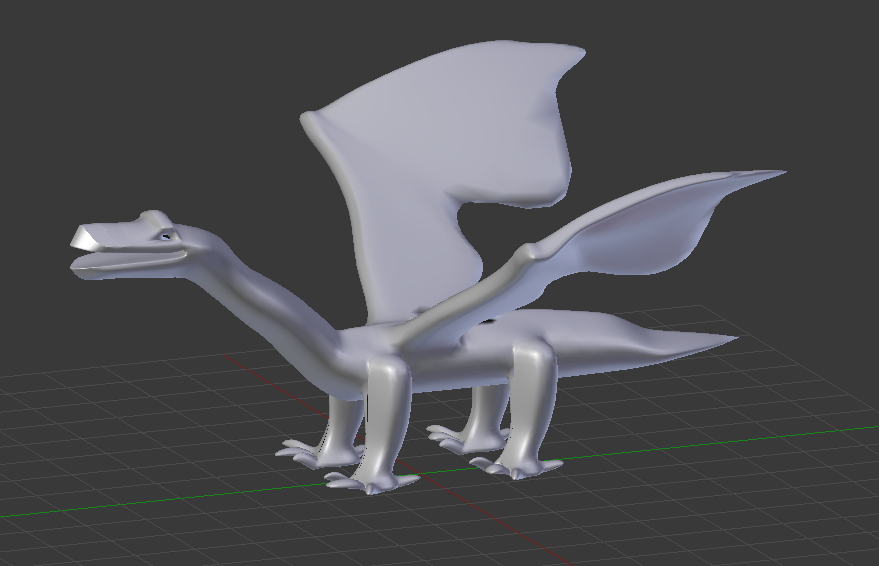
\includegraphics[width=0.6\textwidth]{dragon_front_page.png}
        \vfill
        {\large Printemps 2016}
    \end{center}
\end{titlepage}

\newpage
\tableofcontents
\listoffigures
\newpage
%%%%%%%%%%%%%%%%%%%%%%%%%%%%%%%%%%%%%%%%%%%%%%%%%%%%%%%%%%%%%%%%%%%%%%%%%%%%%%%%%%%%%%%%%%%%%%%%%%%%%%%
\chapter{Présentation du projet}
\par
Durant ce semestre en IN55, nous avons choisi le projet \textit{Animation d'un personnage 3D} parmi tout ceux proposés. Le personnage que nous avons choisi de modéliser et d'animer est un dragon. Les raisons de ce choix sont multiples. 

Tout d'abord, étant tous plus ou moins proche des communautés fan d'heroic-fantasy, le dragon est pour nous une figure emblématique de notre imaginaire. Ce projet nous laisser donc l'opportunité de donner vie à cette créature mythique. 

Dans un second temps, c'est l'architecture du squelette qui nous a donné envie. Basiquement, un dragon c'est : une tête, un cou, un buste, des ailes, des pattes, et une queue. Cette structure nous a paru suffisament complexe pour que l'on puisse faire des animations intéressantes, mais reste relativement simple n'ayant pas forcément trop d'éléments du squelette qui se suivent.

Nous develloperons dans ce rapport la structure de notre objet 3D. Nous parlerons aussi des technologies employées pour faire le rendu 3D et d el'architecture de notre programme. Enfin, nous ouvrirons des pistes d'évolution pour ce projet. 

\newpage
%%%%%%%%%%%%%%%%%%%%%%%%%%%%%%%%%%%%%%%%%%%%%%%%%%%%%%%%%%%%%%%%%%%%%%%%%%%%%%%%%%%%%%%%%%%%%%%%%%%%%%%
\chapter{Modélisation et armature}
\par
Nous avons effectué la modélisation du dragon sous Blender. Son armature se découpe en plusieurs parties indépendantes les unes des autres. Il y a :
\begin{itemize}
\item La tête toute entière
\item La machoire
\item Le cou
\item Le corps allant de la base du coup jusqu'à la queue
\item Les ailes, indépendantes
\item Les pattes, indépendantes également
\end{itemize}

Chaque partie est composée de plusieurs os reliés entre eux. Chaque os dispose d'une position et d'une orientation qui dépends de celle de son parent. Sous Blender nous avons utilisé des Inverse Kinematics Bones pour les pattes et les ailes en particulier. En procédant ainsi, un mouvement fluide est obtenu.

\begin{figure}[H]
    \begin{center}
        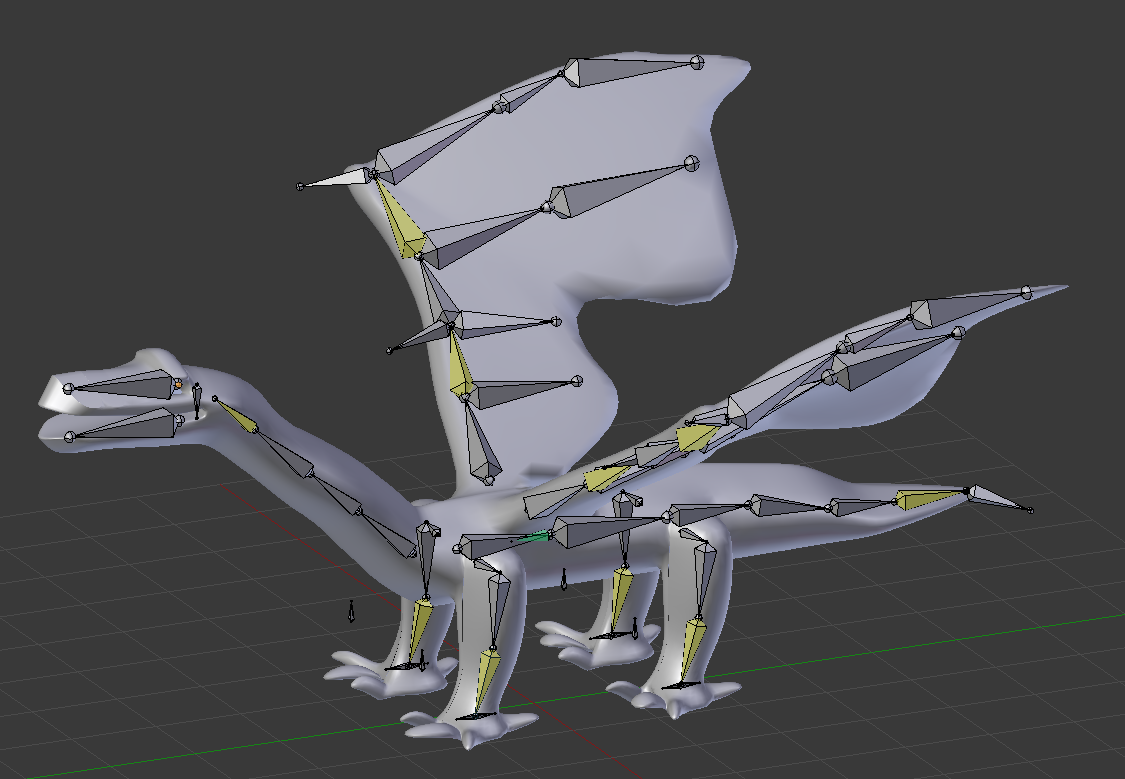
\includegraphics[width=0.85\textwidth]{armature.png}
        \caption{Armature}
    \end{center}
\end{figure}
\newpage
%%%%%%%%%%%%%%%%%%%%%%%%%%%%%%%%%%%%%%%%%%%%%%%%%%%%%%%%%%%%%%%%%%%%%%%%%%%%%%%%%%%%%%%%%%%%%%%%%%%%%%%
\chapter{Diagramme de classe}


\newpage
%%%%%%%%%%%%%%%%%%%%%%%%%%%%%%%%%%%%%%%%%%%%%%%%%%%%%%%%%%%%%%%%%%%%%%%%%%%%%%%%%%%%%%%%%%%%%%%%%%%%%%
\chapter{Architecture du projet}
\section{La librairie Asset Import}
\par
Asset Import est une librairie libre sous licence BSD permettant d'importer dans une structure de données
un très grand nombre de fichiers 3D.
\par
Cela a permis de s'affranchir des opérations bas-niveau de parsage de fichier, ainsi que de la vérification 
syntaxique du fichier 3D, tout en permettant de faire des tests avec un très grand nombre possible de 
fichiers comme le Collada, le FBX, le format 3DS, ou encore simplement un fichier OBJ.
\par
Ces fichiers supportant différentes fonctionnalités, il n'est toutefois pas toujours possible de visualiser
les animations.

\section{Nos structures de données}
\par
Si la librairie assimp permet de charger le fichier en mémoire dans une structure de données, elle ne permet 
cependant pas de faire de l'animation squelettale directement. Il faut donc soit faire une fonction capable 
de parcourir la structure rapidement, afin d'extraire les bonnes informations pour ensuite les afficher, mais
cette solution est très couteuse en terme de temps de calcul, puisqu'en plus de faire les calculs
d'interpolation, il faut aussi gérer le parcours de structure complexe.
\par
Nous avons donc décider de faire nos propres structures de données, plus simples, et donc moins exhaustives,
mais suffisantes pour les besoins du projet.
\par
Des fonctions de chargement sont donc appellées au lancement, récupérant les informations requises grâce à 
assimp, pour pouvoir ensuite y accéder rapidement et simplement.

\subsection{Les structures principales}
\par
On trouve généralement dans un fichier une scène contenant plusieurs objets.

\begin{itemize}
\item $Mesh$ : Un $Mesh$ est une structure qui contient principalement une liste de $vertex$, de $bones$ et de $faces$. L'orientation de ces faces est définie par leur normale, comprise également dans le $mesh$.
\item $Vertice$ : Un $Vertices$ contient un $vertex$ avec deux tableaux de taille 4. Le premier détaille les $Bones$ qui influent sur lui. Le second mesure le poids d'influence.
\item $Bones$ : Un $Bones$ contient un $bone$ et la liste des $vertex$ sur lesquels il influe.
\item $Face$ : Une $Face$ contient une liste d'indice qui forment une face.
\item $Animation$ : Une $Animation$ contient une liste de $BoneAnim$. Il y a autant de liste que de $Bone$.
\item $BoneAnim$ : Une $BoneAnim$ contient 3 listes qui correspondent aux clés pour la translation, la rotation et la mise à l'échelle.
\end{itemize}

%%%%%%%%%%%%%%%%%%%%%%%%%%%%%%%%%%%%%%%%%%%%%%%%%%%%%%%%%%%%%%%%%%%%%%%%%%%%%%%%%%%%%%%%%%%%%%%%%%%%%%
\chapter{Bilan}

\section{Améliorations possibles}
\par
Nous aurions pu améliorer notre projet de la façon suivante :
%brouillon
\begin{itemize}
\item Ajout de textures
\item Système de gestion de lumière avec shader
\item Améliorer les animations, qui restent rudes
\end{itemize}

\section{Conclusion}
\par
Compréhension de la modélisation et l'animation d'un personnage
Représentation du rendu d'une scène
Techniques d'animations, matrice projective

\newpage
%%%%%%%%%%%%%%%%%%%%%%%%%%%%%%%%%%%%%%%%%%%%%%%%%%%%%%%%%%%%%%%%%%%%%%%%%%%%%%%%%%%%%%%%%%%%%%%%%%%%%%
\chapter{Annexes}

\end{document}


